\documentclass[a4paper,11pt]{article}

\renewcommand\bottomfraction{0.9} % default value: 0.3
\renewcommand\textfraction{0.1}   % default value: 0.2

\usepackage{caption}
\usepackage{array}
\usepackage{fullpage, setspace, url}
\usepackage{colortbl}
\usepackage{amsmath}
\usepackage{indentfirst}
%\usepackage{algorithm,algorithmic}
%\definecolor{G6}{rgb}{0.7,0.7,0.7}
%\newcommand{\fc}{\cellcolor{G6}}
\usepackage{subfigure}
\usepackage{multirow}
\usepackage[table]{xcolor}
\usepackage{graphicx} 
\usepackage{bmpsize}
\usepackage{pgfgantt}

% pacotes malucões
\usepackage{graphicx}
\usepackage{amsfonts}
\usepackage{amssymb}
\usepackage{amstext}
\usepackage{hyperref}
\usepackage{ragged2e}
\usepackage{color}
\usepackage{enumerate}
\usepackage{float}
% fonte
\usepackage{helvet}
% coisas de locale
\usepackage[brazil]{babel}
\usepackage[utf8]{inputenc}
\usepackage[T1]{fontenc}
\usepackage{tabularx}

\addtolength{\textwidth}{2cm}
\addtolength{\hoffset}{-1cm}

\addtolength{\textheight}{2cm}
\addtolength{\voffset}{-1cm}

\newcommand{\HRule}{\rule{\linewidth}{0.5mm}}
\newcommand{\DUVIDA}[1]{\huge \textbf {\color{red} #1}\normalsize \\} % escreve uma dúvida grandão vermelha

\begin{document}
% \maketitle

\begin{center}
    \pagestyle{empty} 
    % Upper part of the page
    \textsc{\Large Universidade de São Paulo\\
    Instituto de Ciências Matemáticas e de Computação\\
    SSC0130 - Engenharia de Software - Turma A}\\[5.0cm]

    % Title
    \HRule \\[0.6cm]
    {\Huge Projeto parte 3\\
    Modelagem, Teste e Projeto de Interface}\\[0.4cm]
    \HRule \\[3.5cm]

    % Author and supervisor
    \begin{minipage}{0.45\textwidth}
	    \begin{flushleft} \normalsize
    		\emph{Alunos:}
    		
			\[\begin{array}{lr}
	    		\text{Gil Barbosa Reis} & 8532248 \\
    			\text{Giovane Cunha Mocellin} & 8778382 \\
		    	\text{Leonardo Sampaio Ferraz Ribeiro} & 8532300 \\
				\text{Rogério P. Souza} & 5626341
    		\end{array}\]
    	\end{flushleft}
    \end{minipage}
    \begin{minipage}{0.45\textwidth}
	    \begin{flushright} \normalsize
    		\emph{Professora:} \\
    		Ellen Francine Barbosa
	    \end{flushright}
    \end{minipage}

    \vspace{3.0cm}


    \vfill
    % Bottom of the page
    {\Large São Carlos, SP \\ \today}
    \thispagestyle{empty} 
    \newpage
\end{center}

\pagestyle{plain}
\setcounter{page}{1}
\setstretch{1.2}
\newpage

\tableofcontents
\listoffigures
\newpage

\section{Introdução}
	
\section{Modelagem}

\subsection{Diagrama de Casos de Uso}

O diagrama de casos de uso está representado na figura \ref{diagrama}, incluída no final deste documento.

\subsection{Casos de Uso Expandidos}

\begin{table}[H]
		\begin{tabularx}{\textwidth}{|l|X|}
		\hline
			\textbf{Caso de Uso} &  Gerenciar opiniões sobre Jogo \\ \hline
			\textbf{Atores} &  Usuário  \\ \hline
			\textbf{Finalidade} &  Criar, atualizar ou apagar uma opinião sobre um jogo cadastrado  \\ \hline
			\textbf{Visão Geral} & Usuário clica no botão do gerenciador de opiniões, dentro
da página de um jogo específico ou dentro de sua página de perfil. Alterações são
feitas à opinião. Ao sair, as alterações serão salvas.  \\ \hline
			\textbf{Tipo} &  Secundário e não essencial\\ \hline
			\textbf{Referências Cruzadas} &  R11 \\ \hline
			\textbf{Sequência Típica} & 
			\begin{enumerate}
			\item O usário acessou informações de um jogo e clica no botão de gerenciar opiniões sobre o jogo.
			\item O sistema exibe uma tela onde o usuário pode cadastrar uma opinião, atualizar uma opinião cadastrada por ele ou apagar opinião caso já cadastrada.
			\item O usuário realiza o cadastro da opinião e clica em salvar.
			\item O sistema informa ao usuário que sua opinião foi cadastrada.
			\end{enumerate} \\ \hline
			\textbf{Sequências Alternativas} & 
			\begin{enumerate}
			\item O usuário realiza o cadastro da opinião e clica em salvar.
			\begin{enumerate}
			\item O sistema informa ao usuário que ele não pode cadastrar opinições porque foi bloquear por ter pendências no sistema.
			\end{enumerate}
			\end{enumerate} \\ \hline
		\end{tabularx}
\end{table}

\begin{table}[H]
		\begin{tabularx}{\textwidth}{|l|X|}
		\hline
			\textbf{Caso de Uso} &  Buscar um jogo \\ \hline
			\textbf{Atores} &  Usuário  \\ \hline
			\textbf{Finalidade} &   Buscar um jogo dentre os cadastrados  \\ \hline
			\textbf{Visão Geral} &  Usuário escreve um nome na barra de busca, e clica no botão
de buscar. O sistema mostra todos os resultados da busca.  \\ \hline
			\textbf{Tipo} &   Primário e essencial \\ \hline
			\textbf{Referências Cruzadas} &   R7, R8, R9 \\ \hline
			\textbf{Sequência Típica} & 
			
			\begin{enumerate}
			\item O usuário escreve um nome na barra de busca e pressiona o botão de busca
			
			\item O sistema exibe todos os campos cadastrados que tem relaçao com o nome digitado pelo usuário.
			
			\item O usuário filtra a busca por uma região desejada.
			
			\item O sistema exibe todos os jogos cadastrados da região escolhida pelo usuário.
			
			\item O usuário filtra a busca por título, descrição, gênero, plataformas ou região do jogo e também por classificação de idade.
			
			\item O sistema exibe os jogos cadastrados de acordo com as informações informadas pelo usuário.
			\end{enumerate} \\ \hline
			
			
			\textbf{Sequências Alternativas} & 
						
			\begin{enumerate}
			\item O usuário escreve um nome na barra de busca e pressiona o botão de busca.
			\begin{enumerate}
			\item O sistema exibe a mensagem: nenhum jogo cadastrado com o nome digitado.
			\end{enumerate}
			
			\item O usuário filtra a busca por uma região desejada.												\begin{enumerate}
			\item O sistema exibe a mensagem: nenhum jogo cadastrado na região desejada.
			\end{enumerate}
			
			\item O usuário filtra a busca por título, descrição, gênero, plataformas ou região do jogo e também por classificação de idade.
			\begin{enumerate}
			\item O sistema exibe a mensagem: nenhum jogo cadastrado com as informações desejadas.
			\end{enumerate}
			
			
			\end{enumerate} \\ \hline
			
			
		\end{tabularx}
\end{table}

\begin{table}[H]
		\begin{tabularx}{\textwidth}{|l|X|}
		\hline
			\textbf{Caso de Uso} &  Cadastrar CNPJ \\ \hline
			\textbf{Atores} &  Usuário  \\ \hline
			\textbf{Finalidade} & O usuário deseja se cadastrar no sistema como um patrocinador  \\ \hline
			\textbf{Visão Geral} & O usuário se cadastrou para fazer trocas de jogos e deseja mudar seu perfil para patrocinador cadastrando um CNPJ. \\ \hline
			\textbf{Tipo} & Primário e essencial  \\ \hline
			\textbf{Referências Cruzadas} &  R19 \\ \hline
			\textbf{Sequência Típica} & 
			
			\begin{enumerate}
			\item O usuário acessa a área para editar seu perfil.
			\item O sistema exibe as informações que o usuário pode editar.
			\item O usuário clica em cadastrar como patrocinador.
			\item O sistema exibe a tela de cadastro de Patrocinador.
			\item O usuário informa o CNPJ e a razão social e clica em concluir.
			\item O sistema exibe uma mensagem de cadastrado com sucesso.
			\end{enumerate} \\ \hline
			
			\textbf{Sequências Alternativas} & 
			\begin{enumerate}
			\item O usuário informa o CNPJ e a razão social e clica em concluir.
			\begin{enumerate}
			\item O sistema permance na mesma tela e informa ao usuário que seus dados de cadastro estão incorretos.
			\end{enumerate}
			
			\end{enumerate} \\ \hline
		\end{tabularx}
\end{table}

\begin{table}[H]
		\begin{tabularx}{\textwidth}{|l|X|}
		\hline
			\textbf{Caso de Uso} &  Incluir jogo \\ \hline
			\textbf{Atores} &  Usuário \\ \hline
			\textbf{Finalidade} &  O usuário deseja cadastrar um jogo para realizar uma transação \\ \hline
			\textbf{Visão Geral} &  O usuário clica no botão de cadastro de jogos para trocas, informa ao sistema os dados necessários do jogo e ao salvar as informações caso o jogo for novo são enviadas para a aprovação do administrador do sistema ou apenas são salvas no sistema em caso do jogo já existir. \\ \hline
			\textbf{Tipo} & Primário e essencial \\ \hline
			\textbf{Referências Cruzadas} & R10 \\ \hline
			\textbf{Sequência Típica} & 
			\begin{enumerate}
			\item O usuário acessa a área de cadastro de novos jogos
			\item O sistema exibe o formulário de cadastro de novos jogos
			\item O usuário informa os campos: título, descrição, gênero, plataformas ou região do jogo e também a classificação de idade e clica em salvar.
			\item O sistema exibe a mensagem de cadastro realizado com sucesso.
						
			
			\end{enumerate} \\ \hline
			\textbf{Sequências Alternativas} & 
			\begin{enumerate}
			\item O usuário informa os campos: título, descrição, gênero, plataformas ou região do jogo e também a classificação de idade e clica em salvar.
			\begin{enumerate}
			\item O sistema permanece na mesma tela e exibe a mensagem de dados inválidos.
			\item Caso de Uso: verificar cadastro de jogo.
			\end{enumerate}
			\end{enumerate} \\ \hline
		\end{tabularx}
\end{table}

\begin{table}[H]
		\begin{tabularx}{\textwidth}{|l|X|}
		\hline
			\textbf{Caso de Uso} &  Alterar senha \\ \hline
			\textbf{Atores} & Usuário  \\ \hline
			\textbf{Finalidade} &  Os usuários desejam fazer a alterção da senha cadastrada no sistema \\ \hline
			\textbf{Visão Geral} & O usário já tem um cadastro e deseja alterar a senha. Após a alterção o sistema salva a alteração no sistema. \\ \hline
			\textbf{Tipo} & Secundário e não essencial \\ \hline
			\textbf{Referências Cruzadas} & R25 \\ \hline
			\textbf{Sequência Típica} & 
			\begin{enumerate}
			\item O usuário acessa a área de edição de dados cadastrados.
			\item O sistema exibe uma tela de edição de dados.
			\item O usuário escolhe a opção alterar senha.
			\item O sistema exibe campos para fazer alterção de senha.
			\item O usuário informa a senha antiga, a nova senha e clica em salvar.
			\item O sistema exibe uma mensagem de senha alterada com sucesso.
			\end{enumerate} \\ \hline
			\textbf{Sequências Alternativas} & 
			\begin{enumerate}
			\item O sistema exibe campos para fazer alterção de senha.
			\begin{enumerate}
			\item O usuário não lembra a senha antiga e desiste de fazer a alterção.
			\end{enumerate}
			\item O usuário informa a senha antiga, a nova senha e clica em salvar.			
			
			\begin{enumerate}
			\item O sistema exibe uma mensagem que a senha antiga está incorreta.
			\end{enumerate}
			
			\item O usuário informa a senha antiga, a nova senha e clica em salvar.			
			
			\begin{enumerate}
			\item O sistema exibe uma mensagem informando que a nova senha é inválida.
			\end{enumerate}			
			
			\end{enumerate} \\ \hline
		\end{tabularx}
\end{table}

\begin{table}[H]
		\begin{tabularx}{\textwidth}{|l|X|}
		\hline
			\textbf{Caso de Uso} &  Efetuar login \\ \hline
			\textbf{Atores} &  Usuário  \\ \hline
			\textbf{Finalidade} & Os usuários desejam acessar o seu perfil cadastrado para realizar tarefas de acordo com seu perfil.  \\ \hline
			\textbf{Visão Geral} & Os usuários já tem um cadastro e desejam acessar o sistema para realizar uma atividade. O sistema confere o login e senha do usuário e permite o acesso. \\ \hline
			\textbf{Tipo} &  Primária e essencial. \\ \hline
			\textbf{Referências Cruzadas} & R24 \\ \hline
			\textbf{Sequência Típica} & 
			\begin{enumerate}
			\item O usuário acessa a página do T Play e clica no botão entre.
			\item O sistema exibe o formulário de login.
			\item O usuário preenche os campos com seu login e senha e clica em acessar.
			\item O sistema é redirecionado para a página inicial do usuário.
			\end{enumerate} \\ \hline
			\textbf{Sequências Alternativas} & 
			\begin{enumerate}
			\item O usuário preenche os campos com seu login e senha e clica em acessar.
			\begin{enumerate}
			\item O sistema informa que o perfil do usário não foi encontrado.
			\end{enumerate}
			\end{enumerate} \\ \hline
		\end{tabularx}
\end{table}

\begin{table}[H]
		\begin{tabularx}{\textwidth}{|l|X|}
		\hline
			\textbf{Caso de Uso} &  Gerenciar interesse \\ \hline
			\textbf{Atores} & Usuário   \\ \hline
			\textbf{Finalidade} & O usuário deseja cadastrar, atualizar ou excluir informações de interesse no sistema.  \\ \hline
			\textbf{Visão Geral} &  O usuário acessa a área de gerenciar interesses e informa novos, atualiza ou deleta interesses. \\ \hline
			\textbf{Tipo} & Secundário e não essencial \\ \hline
			\textbf{Referências Cruzadas} & ** \\ \hline
			\textbf{Sequência Típica} & 
			\begin{enumerate}
			\item O usuário acessa a área de gerenciar interesses
			\item O sistema exibe uma tela onde o usuário pode alterar as informações de interesse.	
			\item O usuário clica no botão cadastrar novo interesse.
			\item O sistema exibe a tela de cadastro de interesses.
			\item O usuário informa o novo interesse e salva as alterações.
			\item O sistema exibe a mensagem de interesses atualizados com sucesso.
			\end{enumerate} \\ \hline
			\textbf{Sequências Alternativas} & 
			\begin{enumerate}
			\item O sistema exibe uma tela onde o usuário pode alterar as informações de interesse.
			\begin{enumerate}
			\item O usuário desiste de gerenciar os interesses e cancela a operação.
			\end{enumerate}
			\end{enumerate} \\ \hline
		\end{tabularx}
\end{table}

\begin{table}[H]
		\begin{tabularx}{\textwidth}{|l|X|}
		\hline
			\textbf{Caso de Uso} &  Gerenciar oferta \\ \hline
			\textbf{Atores} &  Usuário  \\ \hline
			\textbf{Finalidade} &  O usuário deseja cadastrar, atualizar ou apagar as ofertas que cadastrou. \\ \hline
			\textbf{Visão Geral} & O usuário acessa a área de gerenciamento de ofertas realiza uma atividade de cadastro, atualização ou deleção em uma oferta e após terminar as informações são salvas no sistema. \\ \hline
			\textbf{Tipo} & Primária e essencial. \\ \hline
			\textbf{Referências Cruzadas} & *R10, *R21 \\ \hline
			\textbf{Sequência Típica} & 
			\begin{enumerate}
			\item O usuário acessa a área de gerenciamento de ofertas.
			\item O sistema exibe as ofertas cadastras pelo usuário.
			\item O usuário clica no botão de cadastro de nova oferta.
			\item O sistema exibe a tela de cadastro de ofertas.
			\item O usuário preenche as informações sobre a nova oferta e clica em salvar.
			\item O sistema exibe a mensagem de dados cadastrados com sucesso.
			\end{enumerate} \\ \hline
			\textbf{Sequências Alternativas} & 
			\begin{enumerate}
			\item O sistema exibe as ofertas cadastras pelo usuário.
			\begin{enumerate}
			\item O usuário cancela a operação.
			\end{enumerate}
			\item O usuário clica no botão de cadastro de nova oferta.			
			\begin{enumerate}
			\item O sistema permanece na mesma tela e exibe uma mensagem de dados inválidos.
			\end{enumerate}
			\end{enumerate} \\ \hline
		\end{tabularx}
\end{table}

\begin{table}[H]
		\begin{tabularx}{\textwidth}{|l|X|}
		\hline
			\textbf{Caso de Uso} &  Realizar venda \\ \hline
			\textbf{Atores} &  Usuário  \\ \hline
			\textbf{Finalidade} &   \\ \hline
			\textbf{Visão Geral} &  \\ \hline
			\textbf{Tipo} & Primária e essencial. \\ \hline
			\textbf{Referências Cruzadas} &  \\ \hline
			\textbf{Sequência Típica} & 
			\begin{enumerate}
			\item Ter tolerância no cronograma
			\end{enumerate} \\ \hline
			\textbf{Sequências Alternativas} & 
			\begin{enumerate}
			\item Ter tolerância no cronograma
			\begin{enumerate}
			\item Ter tolerância no cronograma
			\end{enumerate}
			\end{enumerate} \\ \hline
		\end{tabularx}
\end{table}

\begin{table}[H]
		\begin{tabularx}{\textwidth}{|l|X|}
		\hline
			\textbf{Caso de Uso} &  Realizar troca \\ \hline
			\textbf{Atores} &  Usuário  \\ \hline
			\textbf{Finalidade} &   \\ \hline
			\textbf{Visão Geral} &  \\ \hline
			\textbf{Tipo} & Primária e essencial. \\ \hline
			\textbf{Referências Cruzadas} &  \\ \hline
			\textbf{Sequência Típica} & 
			\begin{enumerate}
			\item Ter tolerância no cronograma
			\end{enumerate} \\ \hline
			\textbf{Sequências Alternativas} & 
			\begin{enumerate}
			\item Ter tolerância no cronograma
			\begin{enumerate}
			\item Ter tolerância no cronograma
			\end{enumerate}
			\end{enumerate} \\ \hline
		\end{tabularx}
\end{table}

\begin{table}[H]
		\begin{tabularx}{\textwidth}{|l|X|}
		\hline
			\textbf{Caso de Uso} &  Alterar estado da oferta \\ \hline
			\textbf{Atores} &  Usuário  \\ \hline
			\textbf{Finalidade} &   \\ \hline
			\textbf{Visão Geral} &  \\ \hline
			\textbf{Tipo} & Primária e essencial. \\ \hline
			\textbf{Referências Cruzadas} &  \\ \hline
			\textbf{Sequência Típica} & 
			\begin{enumerate}
			\item Ter tolerância no cronograma
			\end{enumerate} \\ \hline
			\textbf{Sequências Alternativas} & 
			\begin{enumerate}
			\item Ter tolerância no cronograma
			\begin{enumerate}
			\item Ter tolerância no cronograma
			\end{enumerate}
			\end{enumerate} \\ \hline
		\end{tabularx}
\end{table}

\begin{table}[H]
		\begin{tabularx}{\textwidth}{|l|X|}
		\hline
			\textbf{Caso de Uso} &  Controlar transação financeira \\ \hline
			\textbf{Atores} &  Administrador, Patrocinador e sistema financeiro  \\ \hline
			\textbf{Finalidade} &   \\ \hline
			\textbf{Visão Geral} &  \\ \hline
			\textbf{Tipo} & Primária e essencial. \\ \hline
			\textbf{Referências Cruzadas} &  \\ \hline
			\textbf{Sequência Típica} & 
			\begin{enumerate}
			\item Ter tolerância no cronograma
			\end{enumerate} \\ \hline
			\textbf{Sequências Alternativas} & 
			\begin{enumerate}
			\item Ter tolerância no cronograma
			\begin{enumerate}
			\item Ter tolerância no cronograma
			\end{enumerate}
			\end{enumerate} \\ \hline
		\end{tabularx}
\end{table}

\begin{table}[H]
		\begin{tabularx}{\textwidth}{|l|X|}
		\hline
			\textbf{Caso de Uso} &  Avaliar transação de compra/troca \\ \hline
			\textbf{Atores} &  Usuário  \\ \hline
			\textbf{Finalidade} &   \\ \hline
			\textbf{Visão Geral} &  \\ \hline
			\textbf{Tipo} &  Primária e essencial. \\ \hline
			\textbf{Referências Cruzadas} &  \\ \hline
			\textbf{Sequência Típica} & 
			\begin{enumerate}
			\item Ter tolerância no cronograma
			\end{enumerate} \\ \hline
			\textbf{Sequências Alternativas} & 
			\begin{enumerate}
			\item Ter tolerância no cronograma
			\begin{enumerate}
			\item Ter tolerância no cronograma
			\end{enumerate}
			\end{enumerate} \\ \hline
		\end{tabularx}
\end{table}

\begin{table}[H]
		\begin{tabularx}{\textwidth}{|l|X|}
		\hline
			\textbf{Caso de Uso} &  Realizar backup do banco de dados \\ \hline
			\textbf{Atores} &  Administrador  \\ \hline
			\textbf{Finalidade} &  O administrador deseja manter os dados seguros realizando um backup de todos os dados do sistema. \\ \hline
			\textbf{Visão Geral} & O adminstrador seleciona a opção de backup do sistema e ao terminar é gerado um arquivo com todos os dados do sistema. \\ \hline
			\textbf{Tipo} & Primária e essencial \\ \hline
			\textbf{Referências Cruzadas} &  R27 \\ \hline
			\textbf{Sequência Típica} & 
			\begin{enumerate}
			\item O administrador acessa a área de realização de backup.
			\item O sistema exibe uma tela onde o administrador pode escolher o tipo de backup desejado.	
			\item O administrador escolhe o tipo do backup e clica no botão realizar backup do sistema.
			\item O sistema exibe uma mensagem de backup realizado com sucesso e disponibiliza o arquivo com o backup.
			\item O administrador faz o download do arquivo e finaliza a operação.
			
			\end{enumerate} \\ \hline
			\textbf{Sequências Alternativas} & 
			\begin{enumerate}
			\item O sistema exibe uma tela onde o administrador pode escolher o tipo de backup desejado.
			\begin{enumerate}
			\item O administrador desiste de fazer o backup e cancela a operação.
			\end{enumerate}
			\end{enumerate} \\ \hline
		\end{tabularx}
\end{table}

\begin{table}[H]
		\begin{tabularx}{\textwidth}{|l|X|}
		\hline
			\textbf{Caso de Uso} &  Acessar relatórios \\ \hline
			\textbf{Atores} &  Administrador  \\ \hline
			\textbf{Finalidade} & O administrador deseja ter controle sobre as transações realizadas no sistema.  \\ \hline
			\textbf{Visão Geral} & O administrador acessa a área de acesso à relatórios e gera um relatório de acordo com o período e tipo desejado. Após gerar o relatório informações são salvas no sistema informando data e tipo de relatórios gerados.  \\ \hline
			\textbf{Tipo} & Secundário e essencial \\ \hline
			\textbf{Referências Cruzadas} & R3  \\ \hline
			\textbf{Sequência Típica} & 
			\begin{enumerate}
			\item O admnistrador clica no botão acessar relatórios.
			\item O sistema exibe a tela de acesso aos relatórios.
			\item O administrador escolhe o tipo de relatório desejado e informa o período.
			\item O sistema exibe uma tela com o relatório escolhido e disponibiliza a opção de impressão.
			\item O sistema salva informações do último relatóro gerado
			\end{enumerate} \\ \hline
			\textbf{Sequências Alternativas} & 
			\begin{enumerate}
			\item O sistema exibe a tela de acesso aos relatórios.
			\begin{enumerate}
			\item administrador cancela a operação.
			\end{enumerate}
			\end{enumerate} \\ \hline
		\end{tabularx}
\end{table}

\begin{table}[H]
		\begin{tabularx}{\textwidth}{|l|X|}
		\hline
			\textbf{Caso de Uso} &  Verificar cadastro do jogo \\ \hline
			\textbf{Atores} &   Adminstrador \\ \hline
			\textbf{Finalidade} &  O administrador recebe uma solicitação de cadastro de novo jogo e deseja aceitar ou recusar o novo cadastro. \\ \hline
			\textbf{Visão Geral} & O administrador recebe a solicitação de novo cadastro através do sistema onde ele pode aceitar ou recussar o novo jogo a após a opção o sistema informa o Gamer sobre a decisão do administrador  \\ \hline
			\textbf{Tipo} & Primária e essencial. \\ \hline
			\textbf{Referências Cruzadas} & R5 \\ \hline
			\textbf{Sequência Típica} & 
			\begin{enumerate}
			\item O administrador recebeu uma solicitação de cadastro de novo jogo e acessa a área de verificar cadastro de jogo.
			\item O sistema exibe uma tela com as informações do jogo que deseja ser cadastrado e as opções de aceitar ou recusar. 
			\item O administrador aceita a nova solicitação de cadastro.
			\item O sistema informa ao administrador que sua avalização foi efetuada com sucesso.
			\item O sistema envia uma mensagem para o usuário que fez o cadastro do jogo relatando a decisão do administrador.
			
			\end{enumerate} \\ \hline
			\textbf{Sequências Alternativas} & 
			\begin{enumerate}
			\item O sistema exibe uma tela com as informações do jogo que deseja ser cadastrado e as opções de aceitar ou recusar.
			\begin{enumerate}
			\item O administrador recusa o novo cadastro.
			\item O sistema informa ao administrador que sua avalização foi efetuada com sucesso.
			\item O sistema envia uma mensagem para o usuário que fez o cadastro do jogo relatando a decisão do administrador.
			\end{enumerate}
			\end{enumerate} \\ \hline
		\end{tabularx}
\end{table}

\begin{table}[H]
		\begin{tabularx}{\textwidth}{|l|X|}
		\hline
			\textbf{Caso de Uso} &  Gerenciar propagandas \\ \hline
			\textbf{Atores} & Patrocinador   \\ \hline
			\textbf{Finalidade} &  O patrocinador deseja cadastrar novas, atualizar ou deletar propagandas do sistema. \\ \hline
			\textbf{Visão Geral} &  O patrocinador acessa a área de gerenciamento de propagandas e faz o cadastro ou atualização ou exclui uma propaganda. Após concluir o gerenciamento as informações são salvas no sistema. \\ \hline
			\textbf{Tipo} & Primária e essencial. \\ \hline
			\textbf{Referências Cruzadas} &  R20 \\ \hline
			\textbf{Sequência Típica} & 
			\begin{enumerate}
			\item O patrocinador clica no botão gerenciar propagandas.
			\item O sistema exibe uma tela para gerenciar as propagandas.
			\item O patrocinador escolhe a opão de cadastrar nova propaganda.
			\item O sistema exibe a tela com as informações para a propaganda e as condições de cadastro.	
			\item O patrocinador preenche todas as informações, concorda com os termos de uso e salva as alterações.
			\item O sistema exibe uma mensagem que o cadastro de propaganda foi realizado com sucesso.
			\end{enumerate} \\ \hline
			\textbf{Sequências Alternativas} & 
			\begin{enumerate}
			\item O sistema exibe a tela com as informações para a propaganda e as condições de cadastro.
			\begin{enumerate}
			\item O patrocinador desiste de fazer o cadastro e cancela a operação.
			\end{enumerate}
			\end{enumerate} \\ \hline
		\end{tabularx}
\end{table}

\begin{table}[H]
		\begin{tabularx}{\textwidth}{|l|X|}
		\hline
			\textbf{Caso de Uso} &  Acessar relateorio de vendas \\ \hline
			\textbf{Atores} &   Patrocinador \\ \hline
			\textbf{Finalidade} & O patrocinador quer verificar o relatório de vendas para um determinado período.  \\ \hline
			\textbf{Visão Geral} &  O patrocinador acessa a área de relatórios de vendas, verifica o relatório e pode fazer a impressão do relatório. O sistema exibe as informações e ao sair cadastra no sistema a data do último relatório gerado.  \\ \hline
			\textbf{Tipo} & Primário e essencial \\ \hline
			\textbf{Referências Cruzadas} & R22 \\ \hline
			\textbf{Sequência Típica} & 
			\begin{enumerate}
			\item O patrocinador acessa a área de controle de vendas.
			\item O sistema exibe a opção de gerar relatório de vendas.
			\item O patrocinador informa o período que deseja gerar o relatório e clicar em gerar.
			\item O sistema exibe o relatório de vendas para o período informado pelo patrocinador.
			\end{enumerate} \\ \hline
			\textbf{Sequências Alternativas} & 
			\begin{enumerate}
			\item O patrocinador informa o período que deseja gerar o relatório e clicar em gerar.
			\begin{enumerate}
			\item O sistema informa que o período desejado é inválido.
			\end{enumerate}
			\end{enumerate} \\ \hline
		\end{tabularx}
\end{table}

\section{Testes}
	\begin{center}
	\begin{table}[H]
		\begin{tabularx}{\textwidth}{c|X|X|X|X}
			\textbf{Caso de teste} & \textbf{Cenário} & \textbf{Opinião} & \textbf{Avaliação} & \textbf{Saída Esperada} \\
			\hline
			1 & Sequência Típica - Cenário de Sucesso & Formato Válido & Formato Válido & Opinião alterada\\ \hline
			2 & Sequência A1 - Opinião inválida & Formato Inválido & Formato Válido & Opinião não alterada\\ \hline
			3 & Sequência A2 - Avaliação inválida & Formato Válido & Formato Inválido & Opinião não alterada\\ \hline
			
		\end{tabularx}
		\caption{Teste Caso de Uso Gerênciar Opiniões}
	\end{table}
	\end{center}
	
	\begin{center}
	\begin{table}[H]
		\begin{tabularx}{\textwidth}{c|X|X|X}
			\textbf{Caso de teste} & \textbf{Cenário} & \textbf{Busca} & \textbf{Saída Esperada} \\
			\hline
			1 & Sequência Típica - Cenário de Sucesso & Formato Válido & Busca realizada\\ \hline
			2 & Sequência A1 - Busca inválida & Formato Inválido & Busca não alterada\\ \hline
			
		\end{tabularx}
		\caption{Teste Caso de Uso Buscar Jogos}
	\end{table}
	\end{center}
	
	\begin{center}
	\begin{table}[H]
		\begin{tabularx}{\textwidth}{c|X|X|X|X|X|X}
			\textbf{Caso de teste} & \textbf{Cenário} & \textbf{Nome} & \textbf{Nascimento} & \textbf{Senha} & \textbf{Confirmação Senha} & \textbf{Saída Esperada} \\
			\hline
			1 & Sequência Típica - Cenário de Sucesso & Formato Válido & Formato Válido & Formato Válido & Formato Válido & Opinião alterada\\ \hline
			2 & Sequência A1 - Opinião inválida & Formato Inválido & Formato Válido & Formato Inválido & Formato Inválido & Opinião não alterada\\ \hline
			3 & Sequência A2 - Avaliação inválida & Formato Válido & Formato Inválido & Formato Inválido & Formato Inválido & Opinião não alterada\\ \hline
			
		\end{tabularx}
		\caption{Teste Caso de Uso Incluir Usuários}
	\end{table}
	\end{center}
	
	\begin{center}
	\begin{table}[H]
		\begin{tabularx}{\textwidth}{c|X|X|X}
			\textbf{Caso de teste} & \textbf{Cenário} & \textbf{CNPJ} & \textbf{Saída Esperada} \\
			\hline
			1 & Sequência Típica - Cenário de Sucesso & Formato Válido & Opinião alterada\\ \hline
			2 & Sequência A1 - Opinião inválida & Formato Inválido & Opinião não alterada\\ \hline
			3 & Sequência A2 - Avaliação inválida & Formato Válido & Opinião não alterada\\ \hline
			
		\end{tabularx}
		\caption{Teste Caso de Uso Cadastrar CNPJ}
	\end{table}
	\end{center}
	
	\begin{center}
	\begin{table}[H]
		\begin{tabularx}{\textwidth}{c|X|X|X|X}
			\textbf{Caso de teste} & \textbf{Cenário} & \textbf{Nome} & \textbf{Descrição} & \textbf{Saída Esperada} \\
			\hline
			1 & Sequência Típica - Cenário de Sucesso & Formato Válido & Formato Válido & Opinião alterada\\ \hline
			2 & Sequência A1 - Opinião inválida & Formato Inválido & Formato Válido & Opinião não alterada\\ \hline
			3 & Sequência A2 - Avaliação inválida & Formato Válido & Formato Inválido & Opinião não alterada\\ \hline
			
		\end{tabularx}
		\caption{Teste Caso de Uso Incluir Jogo}
	\end{table}
	\end{center}
	
	\begin{center}
	\begin{table}[H]
		\begin{tabularx}{\textwidth}{c|X|X|X|X|X}
			\textbf{Caso de teste} & \textbf{Cenário} & \textbf{Senha Antiga} & \textbf{Senha Nova} & \textbf{Confirmação Senha Nova} & \textbf{Saída Esperada} \\
			\hline
			1 & Sequência Típica - Cenário de Sucesso & Formato Válido & Formato Válido & Opinião alterada\\ \hline
			2 & Sequência A1 - Opinião inválida & Formato Inválido & Formato Válido & Opinião não alterada\\ \hline
			3 & Sequência A2 - Avaliação inválida & Formato Válido & Formato Inválido & Opinião não alterada\\ \hline
			
		\end{tabularx}
		\caption{Teste Caso de Uso Alterar Senha}
	\end{table}
	\end{center}
	
	\begin{center}
	\begin{table}[H]
		\begin{tabularx}{\textwidth}{c|X|X|X|X}
			\textbf{Caso de teste} & \textbf{Cenário} & \textbf{E-mail} & \textbf{Senha} & \textbf{Saída Esperada} \\
			\hline
			1 & Sequência Típica - Cenário de Sucesso & Formato Válido & Formato Válido & Opinião alterada\\ \hline
			2 & Sequência A1 - Opinião inválida & Formato Inválido & Formato Válido & Opinião não alterada\\ \hline
			3 & Sequência A2 - Avaliação inválida & Formato Válido & Formato Inválido & Opinião não alterada\\ \hline
			
		\end{tabularx}
		\caption{Teste Caso de Uso Efetuar Login}
	\end{table}
	\end{center}
	
	\begin{center}
	\begin{table}[H]
		\begin{tabularx}{\textwidth}{c|X|X|X|X}
			\textbf{Caso de teste} & \textbf{Cenário} & \textbf{Entrada 1} & \textbf{Entrada 2} & \textbf{Saída Esperada} \\
			\hline
			1 & Sequência Típica - Cenário de Sucesso & Formato Válido & Formato Válido & Opinião alterada\\ \hline
			2 & Sequência A1 - Opinião inválida & Formato Inválido & Formato Válido & Opinião não alterada\\ \hline
			3 & Sequência A2 - Avaliação inválida & Formato Válido & Formato Inválido & Opinião não alterada\\ \hline
			
		\end{tabularx}
		\caption{Teste Caso de Uso Gerenciar Interesse}
	\end{table}
	\end{center}
	
	\begin{center}
	\begin{table}[H]
		\begin{tabularx}{\textwidth}{c|X|X|X|X}
			\textbf{Caso de teste} & \textbf{Cenário} & \textbf{Entrada 1} & \textbf{Entrada 2} & \textbf{Saída Esperada} \\
			\hline
			1 & Sequência Típica - Cenário de Sucesso & Formato Válido & Formato Válido & Opinião alterada\\ \hline
			2 & Sequência A1 - Opinião inválida & Formato Inválido & Formato Válido & Opinião não alterada\\ \hline
			3 & Sequência A2 - Avaliação inválida & Formato Válido & Formato Inválido & Opinião não alterada\\ \hline
			
		\end{tabularx}
		\caption{Teste Caso de Uso Gerenciar Oferta}
	\end{table}
	\end{center}
	
	\begin{center}
	\begin{table}[H]
		\begin{tabularx}{\textwidth}{c|X|X|X|X}
			\textbf{Caso de teste} & \textbf{Cenário} & \textbf{Entrada 1} & \textbf{Entrada 2} & \textbf{Saída Esperada} \\
			\hline
			1 & Sequência Típica - Cenário de Sucesso & Formato Válido & Formato Válido & Opinião alterada\\ \hline
			2 & Sequência A1 - Opinião inválida & Formato Inválido & Formato Válido & Opinião não alterada\\ \hline
			3 & Sequência A2 - Avaliação inválida & Formato Válido & Formato Inválido & Opinião não alterada\\ \hline
			
		\end{tabularx}
		\caption{Teste Caso de Uso Realizar Venda}
	\end{table}
	\end{center}
	
	\begin{center}
	\begin{table}[H]
		\begin{tabularx}{\textwidth}{c|X|X|X|X}
			\textbf{Caso de teste} & \textbf{Cenário} & \textbf{Entrada 1} & \textbf{Entrada 2} & \textbf{Saída Esperada} \\
			\hline
			1 & Sequência Típica - Cenário de Sucesso & Formato Válido & Formato Válido & Opinião alterada\\ \hline
			2 & Sequência A1 - Opinião inválida & Formato Inválido & Formato Válido & Opinião não alterada\\ \hline
			3 & Sequência A2 - Avaliação inválida & Formato Válido & Formato Inválido & Opinião não alterada\\ \hline
			
		\end{tabularx}
		\caption{Teste Caso de Uso Controlar Transação Financeira}
	\end{table}
	\end{center}
	
	\begin{center}
	\begin{table}[H]
		\begin{tabularx}{\textwidth}{c|X|X|X|X}
			\textbf{Caso de teste} & \textbf{Cenário} & \textbf{Entrada 1} & \textbf{Entrada 2} & \textbf{Saída Esperada} \\
			\hline
			1 & Sequência Típica - Cenário de Sucesso & Formato Válido & Formato Válido & Opinião alterada\\ \hline
			2 & Sequência A1 - Opinião inválida & Formato Inválido & Formato Válido & Opinião não alterada\\ \hline
			3 & Sequência A2 - Avaliação inválida & Formato Válido & Formato Inválido & Opinião não alterada\\ \hline
			
		\end{tabularx}
		\caption{Teste Caso de Uso Realizar Troca}
	\end{table}
	\end{center}
	
	\begin{center}
	\begin{table}[H]
		\begin{tabularx}{\textwidth}{c|X|X|X|X}
			\textbf{Caso de teste} & \textbf{Cenário} & \textbf{Entrada 1} & \textbf{Entrada 2} & \textbf{Saída Esperada} \\
			\hline
			1 & Sequência Típica - Cenário de Sucesso & Formato Válido & Formato Válido & Opinião alterada\\ \hline
			2 & Sequência A1 - Opinião inválida & Formato Inválido & Formato Válido & Opinião não alterada\\ \hline
			3 & Sequência A2 - Avaliação inválida & Formato Válido & Formato Inválido & Opinião não alterada\\ \hline
			
		\end{tabularx}
		\caption{Teste Caso de Uso Alterar estado da oferta}
	\end{table}
	\end{center}
	
	\begin{center}
	\begin{table}[H]
		\begin{tabularx}{\textwidth}{c|X|X|X|X}
			\textbf{Caso de teste} & \textbf{Cenário} & \textbf{Entrada 1} & \textbf{Entrada 2} & \textbf{Saída Esperada} \\
			\hline
			1 & Sequência Típica - Cenário de Sucesso & Formato Válido & Formato Válido & Opinião alterada\\ \hline
			2 & Sequência A1 - Opinião inválida & Formato Inválido & Formato Válido & Opinião não alterada\\ \hline
			3 & Sequência A2 - Avaliação inválida & Formato Válido & Formato Inválido & Opinião não alterada\\ \hline
			
		\end{tabularx}
		\caption{Teste Caso de Uso Avaliar transação de compra/troca}
	\end{table}
	\end{center}
	
	\begin{center}
	\begin{table}[H]
		\begin{tabularx}{\textwidth}{c|X|X|X|X}
			\textbf{Caso de teste} & \textbf{Cenário} & \textbf{Entrada 1} & \textbf{Entrada 2} & \textbf{Saída Esperada} \\
			\hline
			1 & Sequência Típica - Cenário de Sucesso & Formato Válido & Formato Válido & Opinião alterada\\ \hline
			2 & Sequência A1 - Opinião inválida & Formato Inválido & Formato Válido & Opinião não alterada\\ \hline
			3 & Sequência A2 - Avaliação inválida & Formato Válido & Formato Inválido & Opinião não alterada\\ \hline
			
		\end{tabularx}
		\caption{Teste Caso de Uso Realizar Backups do Banco de Dados}
	\end{table}
	\end{center}
	
	\begin{center}
	\begin{table}[H]
		\begin{tabularx}{\textwidth}{c|X|X|X|X}
			\textbf{Caso de teste} & \textbf{Cenário} & \textbf{Entrada 1} & \textbf{Entrada 2} & \textbf{Saída Esperada} \\
			\hline
			1 & Sequência Típica - Cenário de Sucesso & Formato Válido & Formato Válido & Opinião alterada\\ \hline
			2 & Sequência A1 - Opinião inválida & Formato Inválido & Formato Válido & Opinião não alterada\\ \hline
			3 & Sequência A2 - Avaliação inválida & Formato Válido & Formato Inválido & Opinião não alterada\\ \hline
			
		\end{tabularx}
		\caption{Teste Caso de Uso Acessar Relatórios}
	\end{table}
	\end{center}
	
	\begin{center}
	\begin{table}[H]
		\begin{tabularx}{\textwidth}{c|X|X|X|X}
			\textbf{Caso de teste} & \textbf{Cenário} & \textbf{Entrada 1} & \textbf{Entrada 2} & \textbf{Saída Esperada} \\
			\hline
			1 & Sequência Típica - Cenário de Sucesso & Formato Válido & Formato Válido & Opinião alterada\\ \hline
			2 & Sequência A1 - Opinião inválida & Formato Inválido & Formato Válido & Opinião não alterada\\ \hline
			3 & Sequência A2 - Avaliação inválida & Formato Válido & Formato Inválido & Opinião não alterada\\ \hline
			
		\end{tabularx}
		\caption{Teste Caso de Uso Verificar Cadastro de Jogo}
	\end{table}
	\end{center}
	
	\begin{center}
	\begin{table}[H]
		\begin{tabularx}{\textwidth}{c|X|X|X|X}
			\textbf{Caso de teste} & \textbf{Cenário} & \textbf{Entrada 1} & \textbf{Entrada 2} & \textbf{Saída Esperada} \\
			\hline
			1 & Sequência Típica - Cenário de Sucesso & Formato Válido & Formato Válido & Opinião alterada\\ \hline
			2 & Sequência A1 - Opinião inválida & Formato Inválido & Formato Válido & Opinião não alterada\\ \hline
			3 & Sequência A2 - Avaliação inválida & Formato Válido & Formato Inválido & Opinião não alterada\\ \hline
			
		\end{tabularx}
		\caption{Teste Caso de Uso Gerenciar Propagandas}
	\end{table}
	\end{center}
	
	\begin{center}
	\begin{table}[H]
		\begin{tabularx}{\textwidth}{c|X|X|X|X}
			\textbf{Caso de teste} & \textbf{Cenário} & \textbf{Entrada 1} & \textbf{Entrada 2} & \textbf{Saída Esperada} \\
			\hline
			1 & Sequência Típica - Cenário de Sucesso & Formato Válido & Formato Válido & Opinião alterada\\ \hline
			2 & Sequência A1 - Opinião inválida & Formato Inválido & Formato Válido & Opinião não alterada\\ \hline
			3 & Sequência A2 - Avaliação inválida & Formato Válido & Formato Inválido & Opinião não alterada\\ \hline
			
		\end{tabularx}
		\caption{Teste Caso de Uso AcessarRrelatório de Vendas}
	\end{table}
	\end{center}	
	
\section{Projeto de Interface}

O projeto de interface levou em consideração as principais interações usuário sistema, sendo estes a página inicial (figura \ref{home}), o cadastro e login de usuário (figuras \ref{cadastro} e \ref{login}), busca de jogos (figura \ref{busca}) e venda/troca de jogos (figura \ref{detalhe}).

\begin{figure}[!H]
    		\centering
        	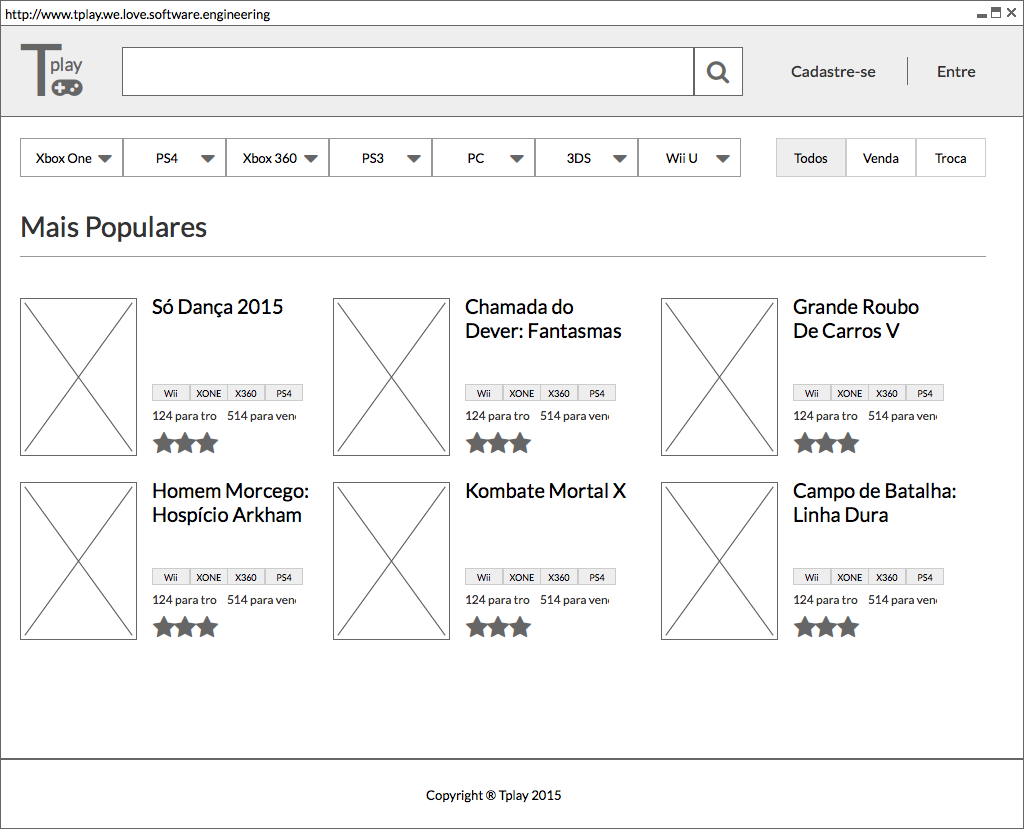
\includegraphics[width=\textwidth,height=\dimexpr\textheight-3\baselineskip\relax,keepaspectratio]{Home.png}
        	\caption{Página inicial do sistema}
     		\label{home}
\end{figure}

\begin{figure}[!H]
    		\centering
        	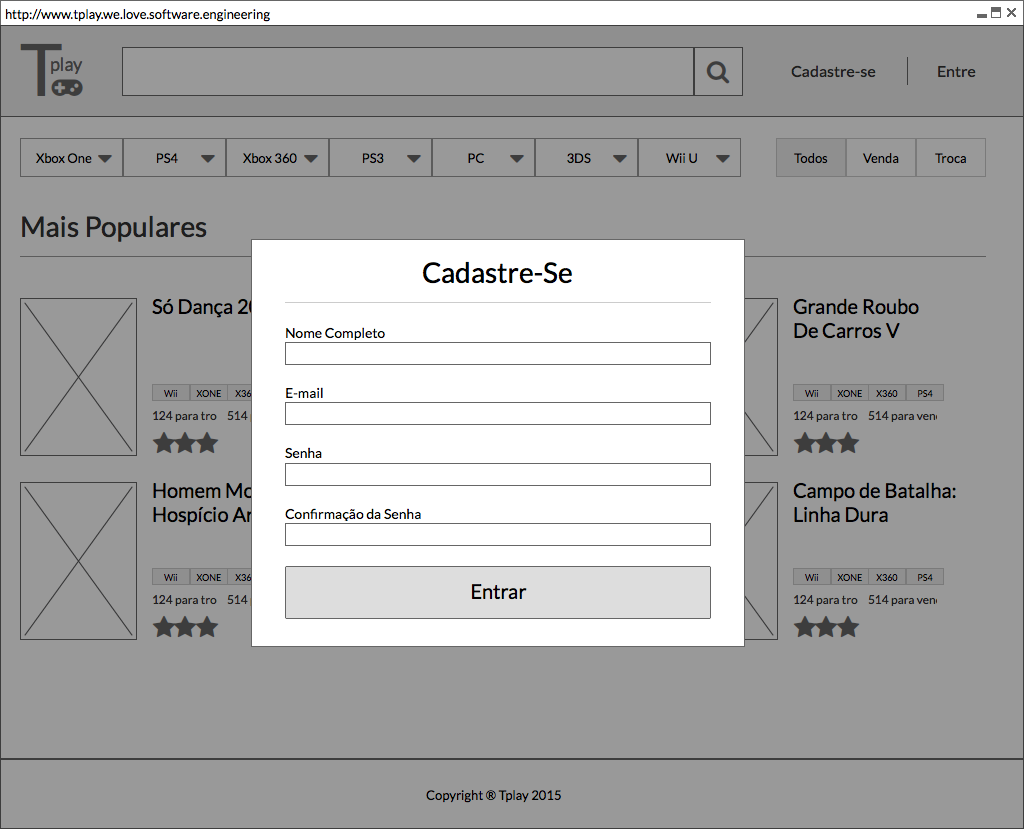
\includegraphics[width=\textwidth,height=\dimexpr\textheight-3\baselineskip\relax,keepaspectratio]{Cadastro.png}
        	\caption{Janela modal de login usuário}
     		\label{cadastro}
\end{figure}

\begin{figure}[!H]
    		\centering
        	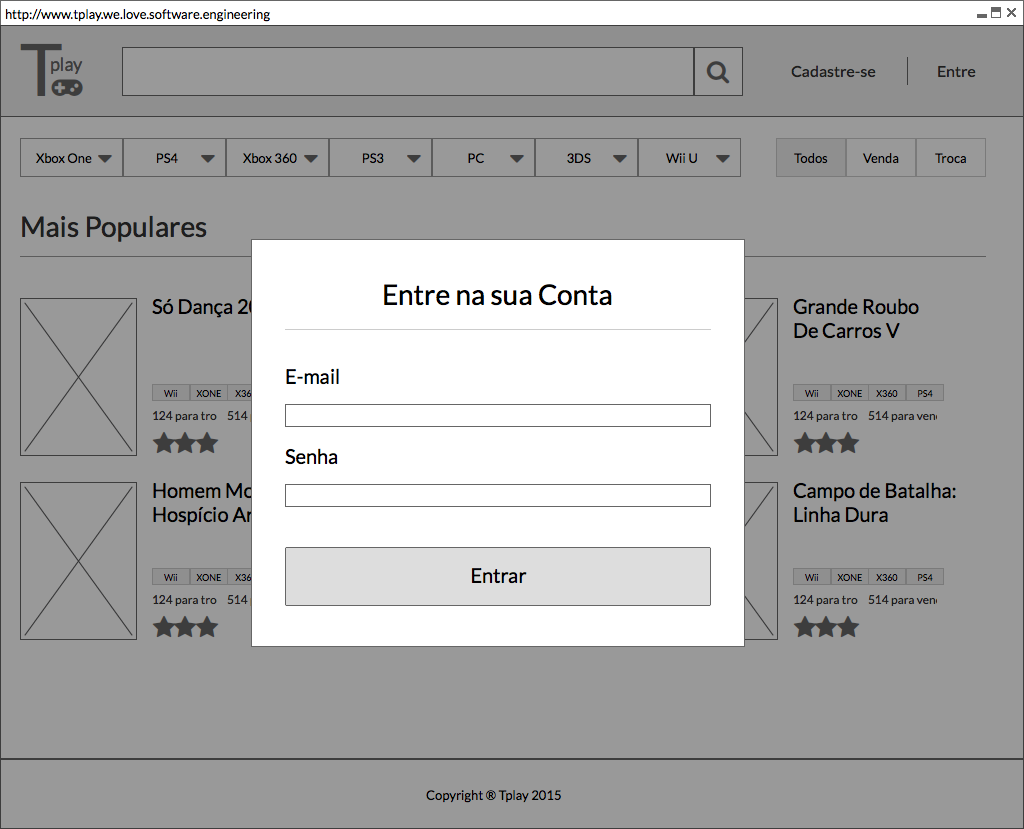
\includegraphics[width=\textwidth,height=\dimexpr\textheight-3\baselineskip\relax,keepaspectratio]{Login.png}
        	\caption{Janela modal de cadastro de novo usuário}
     		\label{login}
\end{figure}

\begin{figure}[!H]
    		\centering
        	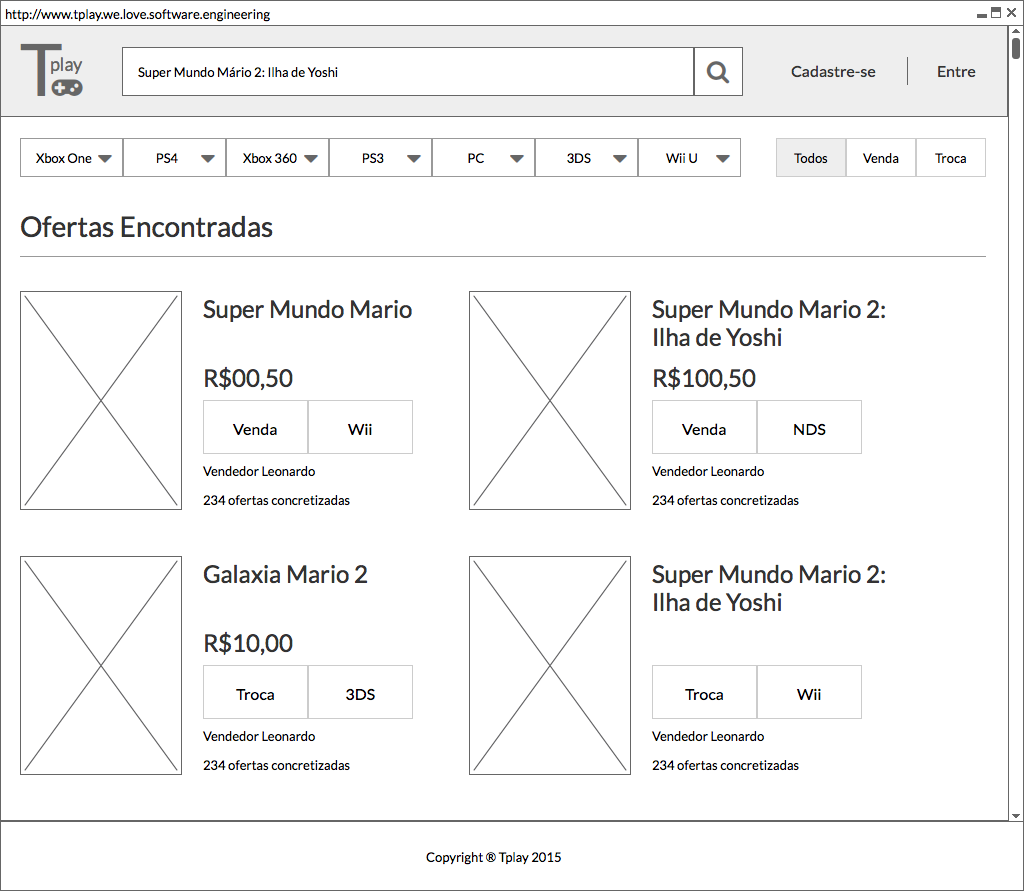
\includegraphics[width=\textwidth,height=\dimexpr\textheight-3\baselineskip\relax,keepaspectratio]{Busca.png}
        	\caption{Resultado de uma busca de jogo}
     		\label{busca}
\end{figure}

\begin{figure}[!H]
    		\centering
        	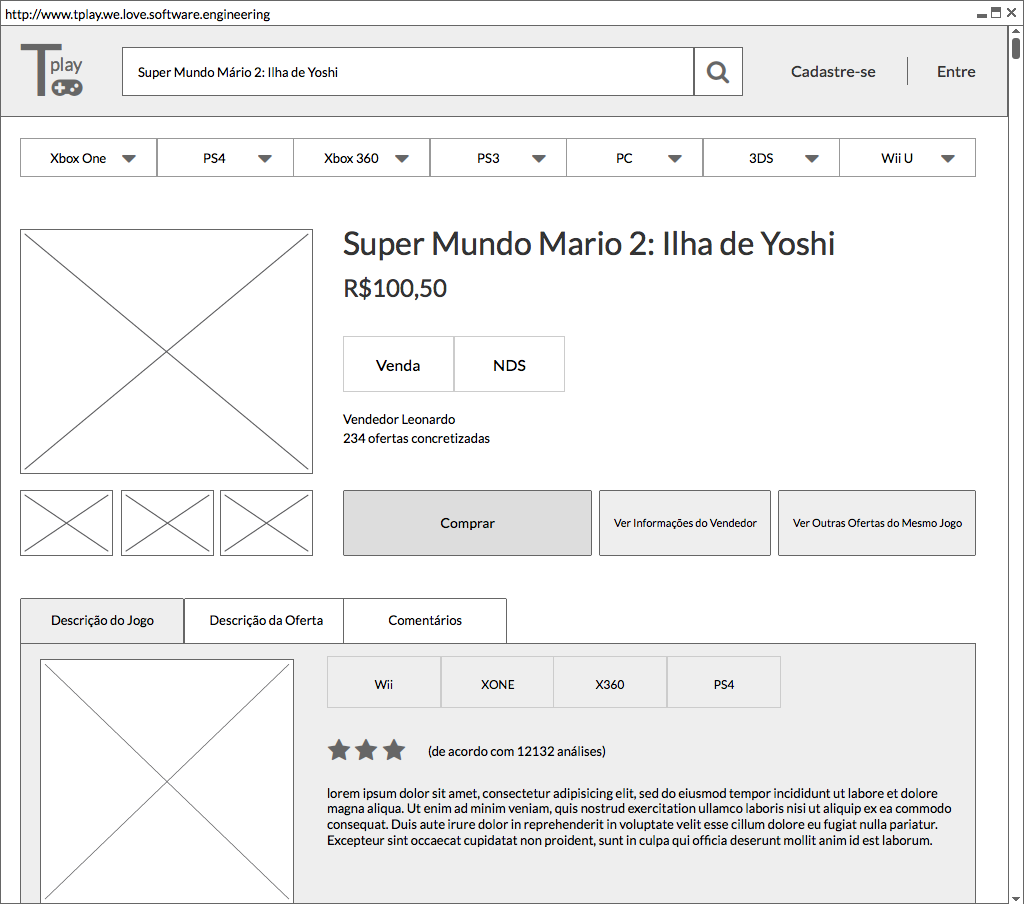
\includegraphics[width=\textwidth,height=\dimexpr\textheight-3\baselineskip\relax,keepaspectratio]{Detalhe.png}
        	\caption{Página de venda ou troca de jogo, com detalhes do jogo e da oferta}
     		\label{detalhe}
\end{figure}

\begin{figure}[!H]
    		\centering
        	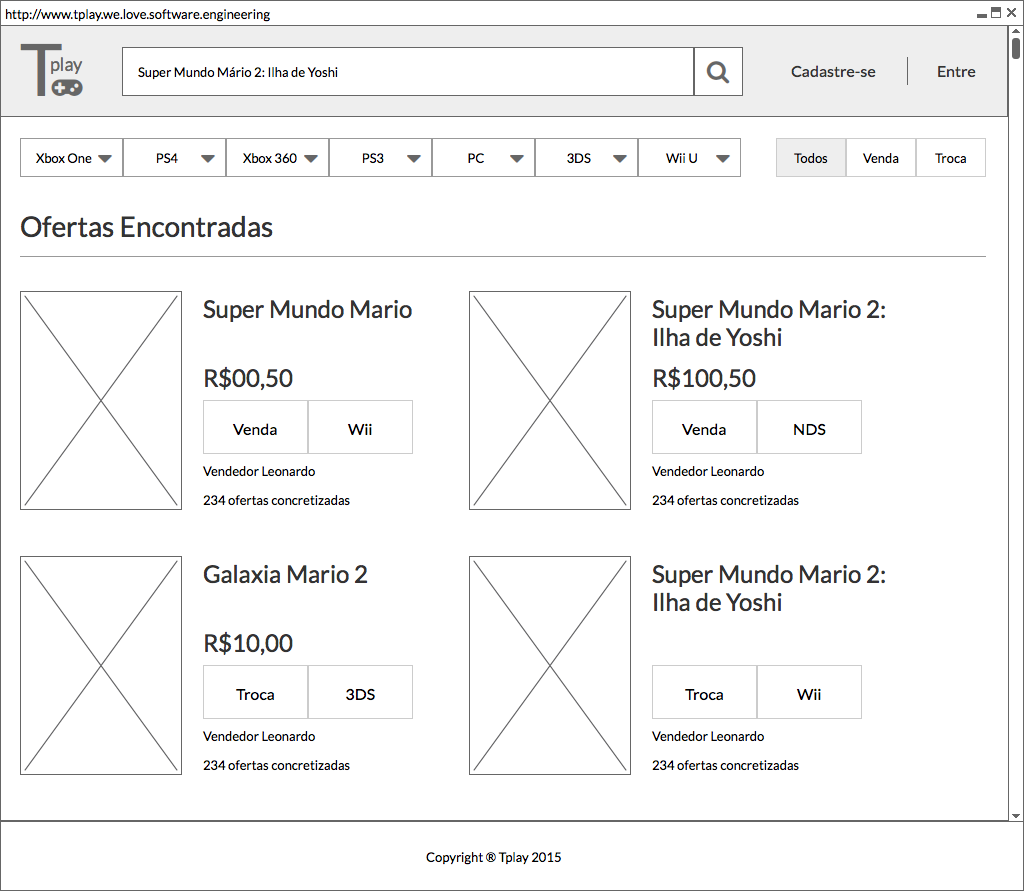
\includegraphics[width=\textwidth,height=\dimexpr\textheight-3\baselineskip\relax,keepaspectratio]{Busca.png}
        	\caption{Resultado de uma busca de jogo}
     		\label{diagrama}
\end{figure}

\section{Conclusão}

\begin{figure}[!H]
    		\centering
        	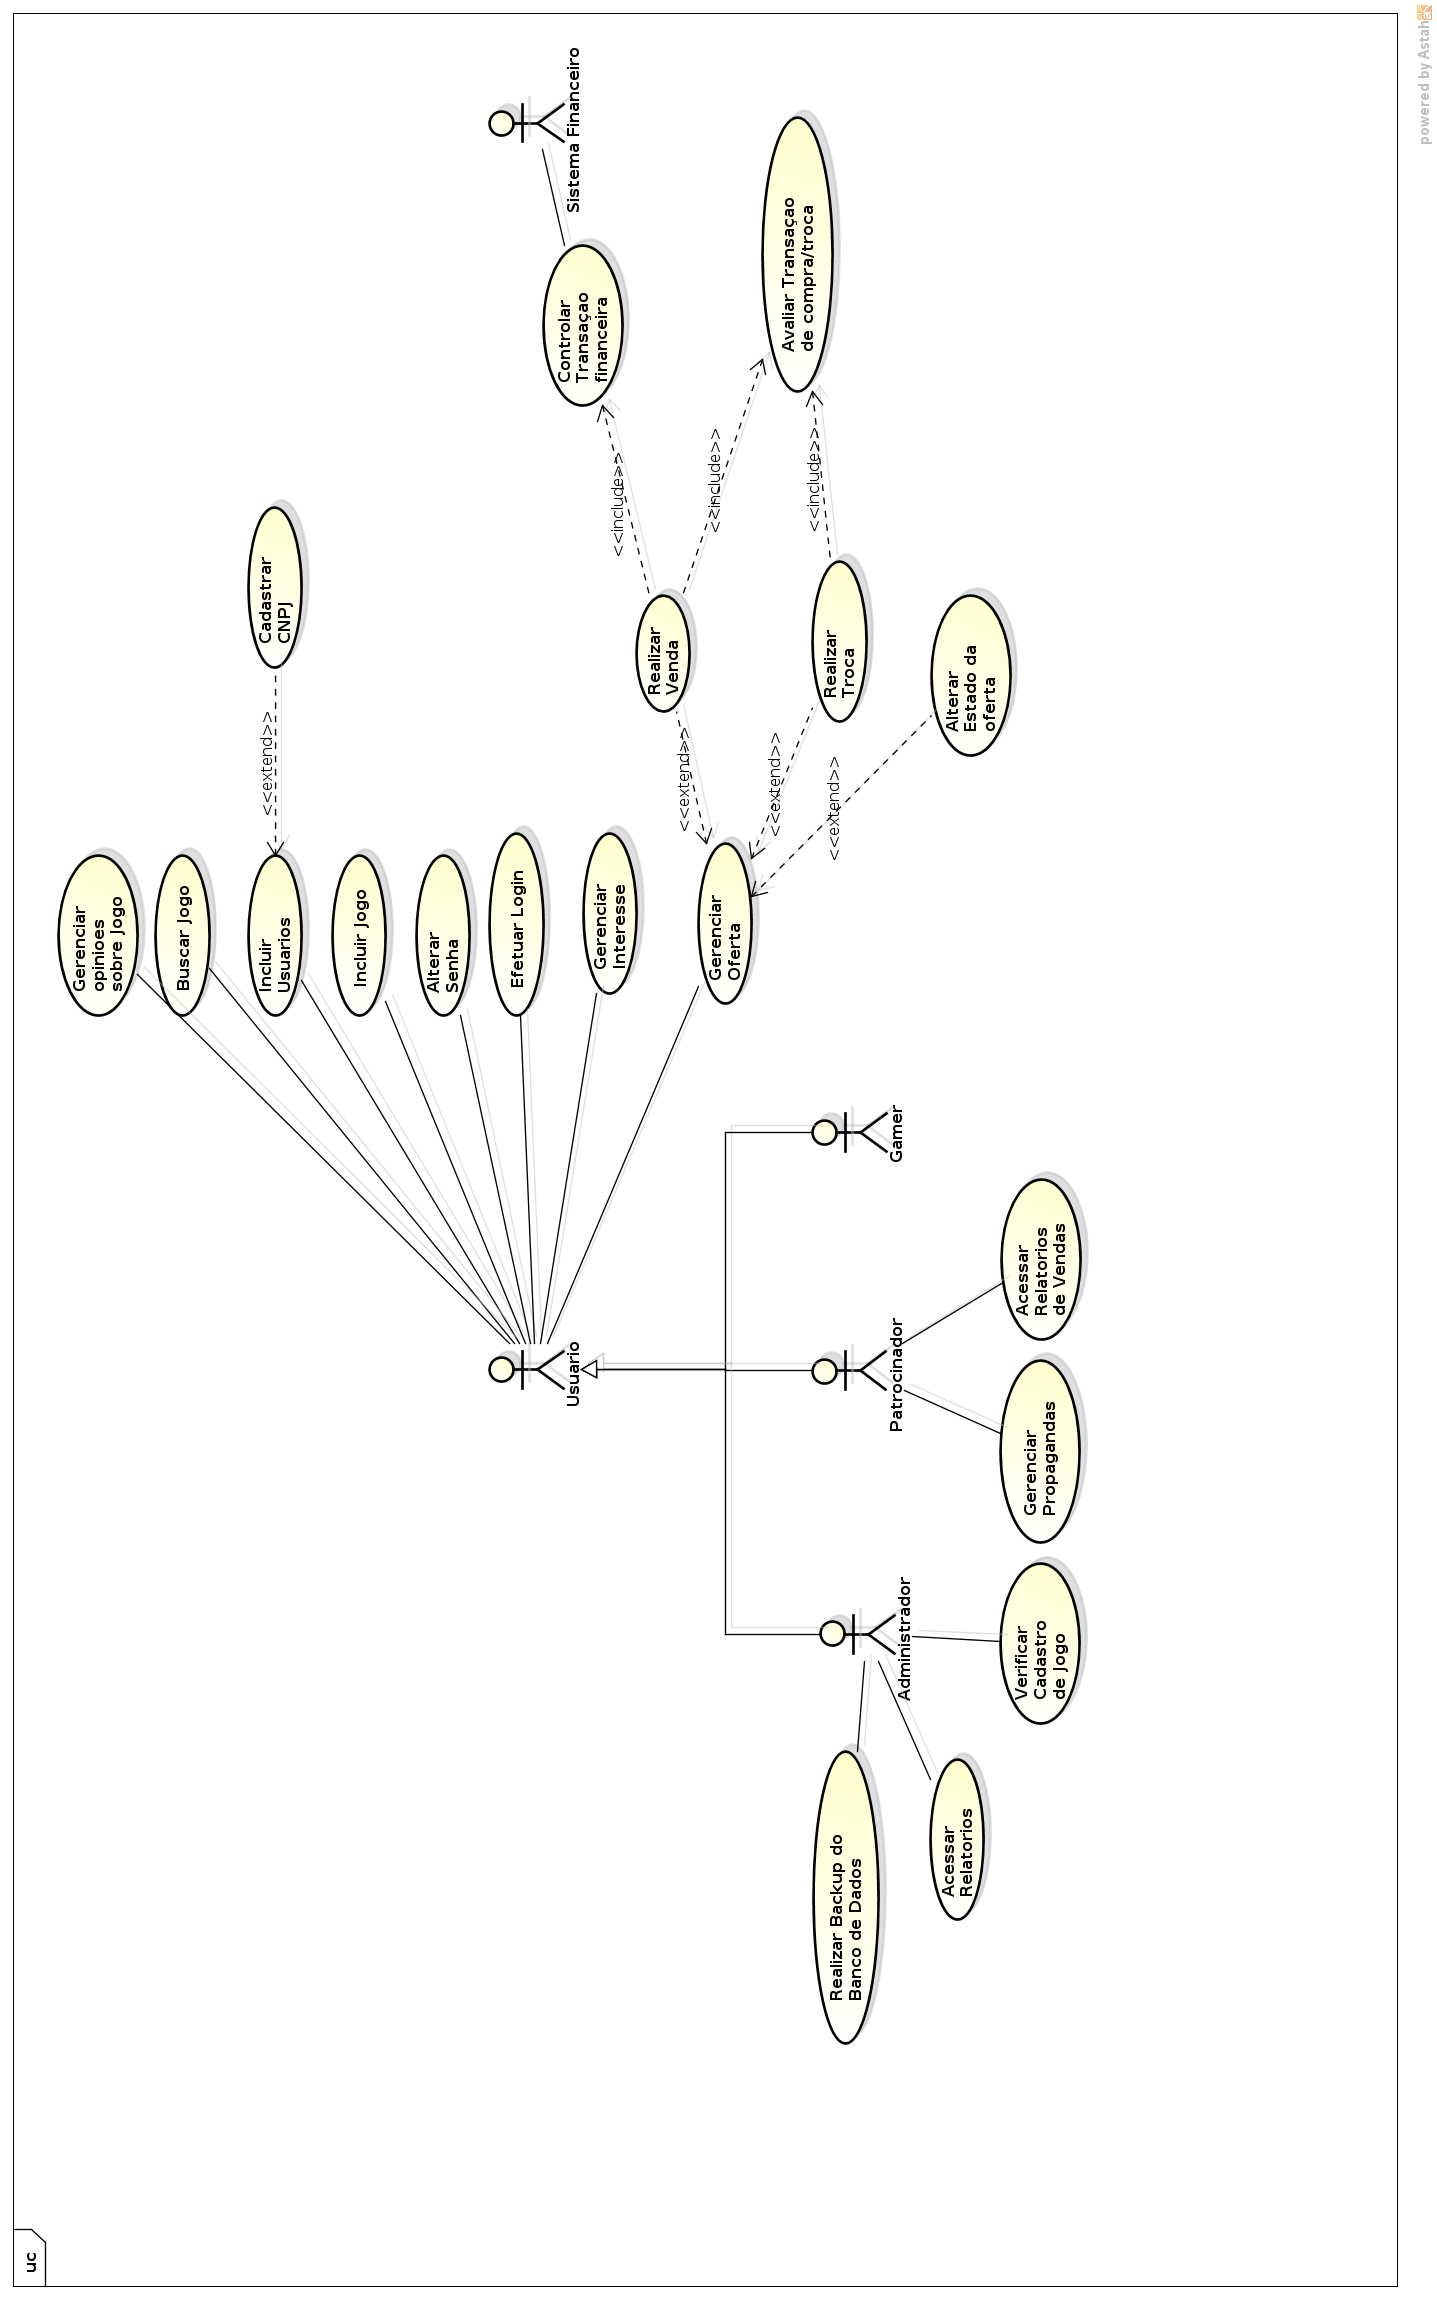
\includegraphics[width=\textwidth,height=\dimexpr\textheight-3\baselineskip\relax,keepaspectratio]{Diagrama.png}
        	\caption{Diagrama de Casos de Uso}
     		\label{diagrama}
\end{figure}
    	

\end{document}
